\documentclass[a4paper, openany]{memoir}

\usepackage[utf8]{inputenc}
\usepackage[T1]{fontenc} 
\usepackage[english]{babel}

\usepackage{fancyhdr}
\usepackage{float}

\usepackage{amsmath}
\usepackage{amsthm}
\usepackage{amssymb}
\usepackage{enumitem}
\usepackage{multicol}
\usepackage[bookmarksopen=true,bookmarksopenlevel=2]{hyperref}
\usepackage{tikz}
\usepackage{indentfirst}

\pagestyle{fancy}
\fancyhf{}
\fancyhead[LE]{\leftmark}
\fancyhead[RO]{\rightmark}
\fancyhead[RE, LO]{Data Fundamentals}
\fancyfoot[LE, RO]{\thepage}
\fancyfoot[RE, LO]{Pete Gautam}

\renewcommand{\headrulewidth}{1.5pt}

\chapterstyle{thatcher}
\setcounter{chapter}{4}
\begin{document}
\chapter{Probability}
\section{Introduction to probability}
Probability is concerned with stochastic elements- the role of uncertainty, randomness and statistics in computation. The study of probability is called probability theory. It allows us to deal with uncertain values and infer the most likely hypothesis from the observations.

The following terms are used in probability theory:
\begin{itemize}
    \item Experiment/trial: an occurrence of an uncertain outcome;
    \item Outcome: the result of an experiment/one state of the world;
    \item Sample space: all the possible outcomes of an experiment;
    \item Event: a subset of possible outcomes with some common property;
    \item Probability: the probability of an event with respect to the sample space is the number of outcomes from the sample space that are in the event, divided by the total number of outcomes in the sample space. Since it is a ratio, it will be a number between 0 (impossible event) and 1 (certain event).
    \item Probability distribution: A mapping of the outcomes to probabilities. The sum of the probability distributions is 1- a trial must result in an outcome (with probability 1), so of all the possible outcomes is 1. A random variable has a probability distribution that maps each outcome to a probability.
    \item Random variable: A variable representing an unknown value, whose probability distribution we know. The variable is associated outcomes from a trial.
    \item Probability density/mass function: A function that defines probability distribution by mapping each outcome to a probability, i.e. $f_X(x) \to \mathbb{R}$. This function could be continuously (density), or discrete (mass) with respect to $x$.
    \item Observation: An outcome we have observed directly, i.e. the dataset.
    \item Sample: An outcome we have simulated according to a probability distribution.
    \item Expectation/expected value: The average value of a random variable.
\end{itemize}

In words, a random variable $X$ has probability distribution $P(X)$, which assigns probabilities $0 \leq P(X = x) \leq 1$ to outcomes $x$, which belong in some sample space $\mathbf{x}$. The probability distribution is defined by a probability mass/density function $f_X(x)$ which assigns probabilities to outcomes such that the sum of probabilities over all the possible outcomes
\[\sum_{x \in X} f_X(x) = 1.\]
We can observe specific outcomes $x_i$ drawn from a distribution as a result of trials. We can sample new outcomes $x_j'$ given a distribution $P(X)$. Assuming outcomes have values, we can evaluate the average expected value $E[X]$ across infinitely many trials.
\newpage

\section{Philosophy of probability}
There are two types of probability- Bayesian and Frequentist.

\subsection{Bayesian probability}
Bayesian probability is the calculus of belief. In this model, probabilities are measured in degrees of belief. $P(A) = 0$ means that the event cannot be true, and $P(A) = 1$ means that the event is certain. It makes sense, in Bayesian perspective, to say that the chance of rain today is $0.3$ (even though this is a one-off event). Moreover, this doesn't mean that it is raining $30\%$; it means that we expect it to rain with confidence $30\%$ due of some hypotheses.

In the Bayesian perspective, we are updating our beliefs. There are 3 aspects to it:
\begin{itemize}
    \item prior belief (what we already know from previous observations),
    \item new evidence (the data we are observing at the moment), and
    \item updating our belief to compute the posterior.
\end{itemize}
\noindent Bayesian inference requires that we accept priors over events, i.e. that we must explicitly quantify our assumptions with probability distributions. It is an extension of logic to uncertain information.

\subsection{Frequentist probability}
On the other hand, under frequentist probability, we only consider the long-term behaviour of repeated events, e.g. the probability of a coin coming up heads in 0.5 because over the long term, this will be the average proportion of times this occurs. It does not make sense in the world view to talk about the probability of events that can only happen in once.

Bayesian probability theory is sometimes said to be subjective because it requires the specification of prior belief, whereas frequentist models of probability do not admit the concept of priors and thus is objective.

Alternatively, the Bayesian model explicitly encodes uncertain knowledge and states universal formal rules for manipulating that knowledge, as formal logic does for definite knowledge. Frequentist methods are objective in the sense that they make statements about universal truths (i.e. the asymptotic behaviour), but they do not form a calculus of belief, and thus can't answer many questions of important directly.

In summary, Bayesian:
\begin{itemize}
    \item includes priors;
    \item probability is a degree of belief;
    \item parameters of populations are considered to be random variables, and data is to be known.
\end{itemize}
On the other hand, Frequentist:
\begin{itemize}
    \item has no priors;
    \item probability is the long-term frequency of events;
    \item parameters of population assumed to be fixed, data to be random.
\end{itemize}
\newpage

\section{Forward and inverse probability}
Generative process is the idea that there is some unknown process going on, the results of which can be observed. The process is governed by some variables that we do not know, but we can infer.

For example, consider the urn problem. We have poured some balls (black and white) into an urn. We can ask the following questions about it:
\begin{itemize}
    \item What is the probability that the next ball will be white? This is a forward probability question- it is a question about the distribution of the observations.
    \item What is the distribution of black and white balls? This is an inverse probability question- these questions depend on unobservable variables that generated these observations.
\end{itemize}

\subsection{Axioms of probability}
The following are the axioms of probability:
\begin{itemize}
    \item the value
    \[0 \leq P(A) \leq 1,\]
    where $A$ is an event- axiom of boundedness.
    
    \item the sum
    \[\sum_A P(A) = 1,\]
    where $A$ is an outcome (single event)- axiom of unitarity.

    \item the sum
    \[P(A \lor B) = P(A) + P(B) - P(A \land B),\]
    where $A$ and $B$ are events- the sum rule.

    \item the conditional probability
    \[P(A|B) = \frac{P(A \land B)}{P(B)},\]
    where $A$ and $B$ are events. $P(A|B)$ refers to the probability of $A$ happening given that $B$ has happened. This is the conditional probability rule.
\end{itemize}

\subsection{Random variables and distributions}
A random variable can take some value, but we do not know what this value is. However, we have some knowledge which captures the possible states the variable could take on, and their corresponding probabilities. A random variable can be:
\begin{itemize}
    \item the outcome of dice throw (discrete);
    \item whether or not it is raining outside (discrete: binary);
    \item the height of person we haven't met yet (continuous).
\end{itemize}

A probability distribution defines how likely different states of random variable are. We can see $X$ as the experiment and $x$ as the outcome, with a function mapping every possible outcome to a probability. We denote $P(X = x)$ for the probability that the random variable $X$ takes the value $x$. The outcome of a random variable can be thought of as taking some value. We write $P(A)$ for the probability of the event $A$, not some random variable $A$.

\subsection{Discrete and continuous distributions}
There are 2 types of random variables:
\begin{itemize}
    \item Discrete variables: the distributions of discrete random variables is given by a probability mass function (PMF). It gives each outcome of a specific value, e.g. a dictionary mapping outcomes to probabilities. It is denoted by $f_X(x)$, where $P(X = x) = f_X(x)$.
    \item Continuous variables: the distribution of continuous random variables is given by a probability density function (PDF). It gives the spread of the probability over outcomes as a continuous function $f_X(x)$. It is not the case that $P(X = x) = f_X(x)$ for PDFs.
\end{itemize}

A PMF or PDF must sum/integrate to 1- the random variable must take some value. This is the unitarity axiom. Every repetition of an experiment has exactly one outcome. Sp, we have
\[\sum_i f_X(x_i) = 1\]
for PMFs , and
\[\int_x f_X(x) \ dx = 1\]
for PDFs.

For example, consider the probability of getting a value between 2 and 12 after two dice rolls. There is only one way to get values $2$ and $12$, so their probability is $\frac{1}{36}$, but there are 6 ways to get a $7$ ($1 + 6$, $2 + 5$, $3 + 4$, $4 + 3$, $5 + 2$ and $6 + 1$), so its probability is $\frac{1}{6}$. The PMF contains the probability of each of the values between 2 and 12. The image below shows the probabilities.
\begin{figure}[H]
    \centering
    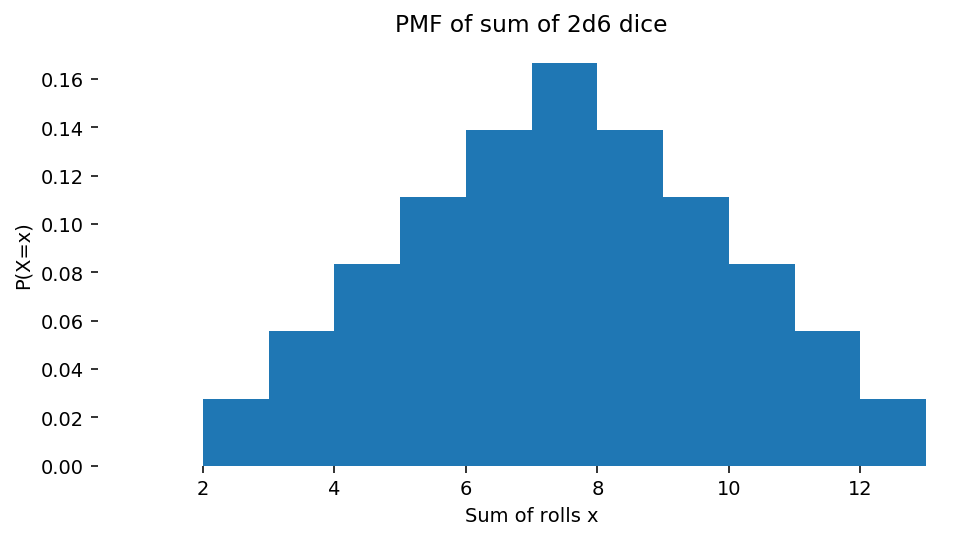
\includegraphics[scale=0.6]{src/5.1 pmf of sum 2d6 dice.png}
    \caption{The PMF of two dice rolls.}
\end{figure}
\newpage

\section{Expectation}
If a random variable takes on numerical values, then we define the  expected value/expectation of a random variable by
\[E[X] = \int_x xf_X(x) \ dx.\]
For a discrete random variable, we have
\[E[X] = \sum_x xf(x).\]
In particular, if there are only finite possiblities, then
\[E[X] = P(X = x_1) x_1 + P(X = x_2) x_2 + \dots + P(X = x_n) x_n.\]
The expectation is the average value of the random variable- the outcome we expect to happen. For example, the expected value of the sum of two dice is 7.

Expectation corresponds to the mean- it is the true average of the value of all the outcomes that would be observed if we ran the experiment an infinite number of times. This is the population mean. So, the mean of a random variable is $E[X]$- it is a measure of the central tendency. Also, the variation of a random variable is $E[X - E[X]^2]$- it is a measure of spread.

We can apply a function to random variables, e.g. square of a random variable. Moreover, if $g(X)$ is a continuous random variable $X$, then
\[E[g(X)] = \int_x f_X(x) g(x) \ dx,\]
or
\[E[g(x)] = \sum_x f_x(x) g(x)\]
for a discrete random variable. For example, the expected value of the square of the sum of two dice is 54.83. Note that $E[g(X)] \neq g(E[X])$. The expected value of the square of the sum of two dice is not $7^2 = 49$, but instead 54.83. So, we have to apply the function to the random variable before multiplying by the probability mass function.

% We can compute the expectation of a two-dice game, where one gets 10 points if the two dice roll the same number, and 0 otherwise (pairs of nothing game). We apply this as a function to the PMF.

Expected values are essential in making rational decisions, the central problem of decision theory. They combine scores (or utility) with uncertainty (probability).
\newpage

\section{Samples and sampling}
Samples (or observations) are observed outcomes form an experiment. We can sample from a distribution. This involves simulating outcoms according to the probability distribution. For example, we can sample from the sum of dice PMF by rolling two dice and summing the result. This is a sample or a draw from the distribution. For discrete random variables, this is easy- we simply produce samples by drawing each outcome according to its probability.

The PMF we estimate by using the observations for discrete random variables is called the empirical distribution. The empirical distribution is given by
\[P(X = x) = \frac{n_x}{N},\]
where $n_x$ is the number of times that value $x$ was observed, and $N$ is the total number of trials. As the number of trials increases, the empirical distribution gets closer to the true PMF, assuming that we are sampling in a non-biased way. For example, using 100 samples, the empirical PMF for two dice rolls is:
\begin{figure}[H]
    \centering
    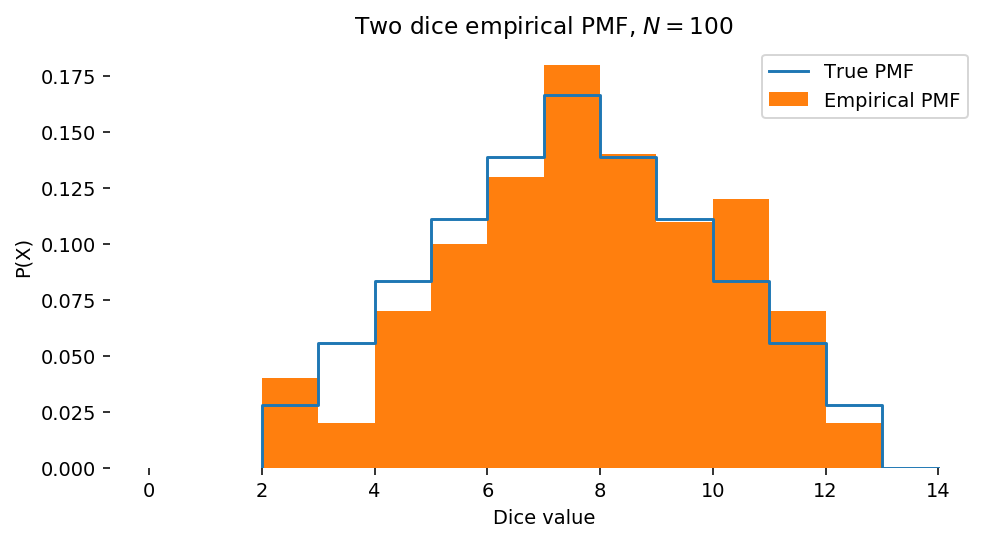
\includegraphics[scale=0.6]{src/5.2 two dice empirical pmf.png}
    \caption{Two dice empirical PMF.}
\end{figure}

\subsection{Uniform sampling}
There are algorithms that can return (pseudo-)random numbers uniformly distributed in some interval, e.g. between 0 and 1. A uniformly distributed number has equal probability of taking any value in the interval, and zero probability everywhere else. Although this is sampling from a continuous PDF, it is the key building block in sampling from arbitrary PMFs. It is denoted by $X \sim U(a, b)$, where $X$ is a random variable that can take values between $a$ and $b$, with equal possibility for any number in that interval. The symbol $\sim$ means distributed as, i.e. ``$X$ is distributed as a uniform distribution in the interval $[a, b]$''.

\subsection{Discrete Sampling}
For a discrete PMF, we can sample outcomes by partitioning the unit interval. To do this, we first choose an arbitrary ordering of the outcomes $x_1, x_2, \dots$ (the data is normally ordered if it is an array, for example). We assign each outcome to a ``bin'', which is a portion of the interval $[0, 1]$ so that the interval is divided into consecutive, non-overlapping intervals. We draw a uniform sample from $[0, 1]$. Then, whichever ``outcome bin'' it lands in is the sample to draw (this is done using \texttt{np.digitize(samples, cmf)}). Since the cumulative sum of the arbitrary order will have last entry 1 (the total sum of all the outcomes is 1), we can sample using the interval $[0, 1]$.

For example, assume that our PMF has 4 word choices: \texttt{cat} with probability 0.28, \texttt{dog} with probability 0.5, \texttt{sheep} with probabilty 0.2, and \texttt{dragon} with probability 0.02. Then, discrete sampling gives us the following.
\begin{figure}[H]
    \centering
    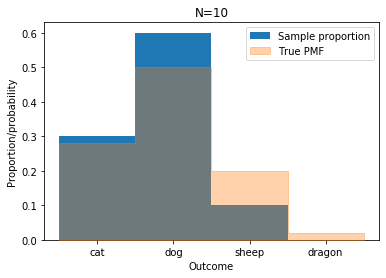
\includegraphics[scale=0.5]{src/5.3 emprical 10.png}
    \caption{Empirical sampling with 10 samples}
\end{figure}
\begin{figure}[H]
    \centering
    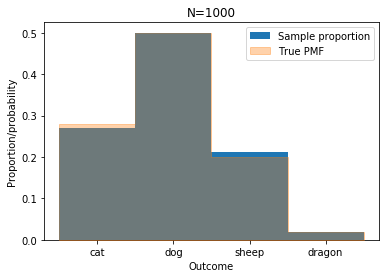
\includegraphics[scale=0.5]{src/5.4 empirical 1000.png}
    \caption{Empirical sampling with 1000 samples}
\end{figure}
\noindent Clearly, as the number of samples increases, the emprical PMF gets closer to the true PMF.

We will look at another example. Consider the likelihood of characters in different texts. We will look at 2 texts- Romeo and Juliet and Metamorphosis:
\begin{figure}[H]
    \centering
    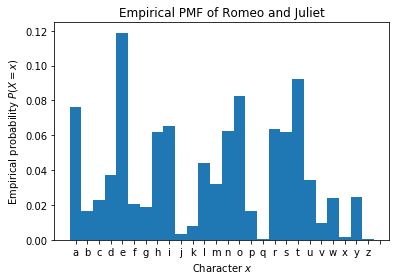
\includegraphics[scale=0.5]{src/5.5 empirical pmf Romeo Juliet.png}
    \caption{Empirical PMF for Romeo and Juliet}
\end{figure}
\begin{figure}[H]
    \centering
    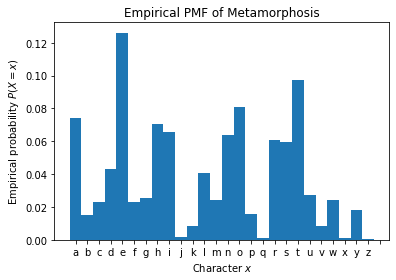
\includegraphics[scale=0.5]{src/5.6 empirical pmf Metamorphosis.png}
    \caption{Empirical PMF for Metamorphosis}
\end{figure}
\noindent The two texts were written by two different authors, and so have somewhat different empirical PMFs. Nonetheless, they are quite similar since both texts are in English.
\newpage

\section{Joint, Conditional and Marginal}
The joint probability of two probabilities is written $P(X, Y)$. It denotes the probability that both $X$ and $Y$ take the specific value at the same time, i.e. $P(X = x) \land P(Y = y)$. The marginal probability is finding $P(X)$ using $P(X, Y)$- we integrate/sum over all the possible outcomes of $Y$.
\[P(X) = \int_y P(X, Y) \ dy\]
for a PDF, and
\[P(X) = \sum_y P(X, Y)\]
for a PMF. Two random variables are independent if they do not depend on each other. If the variables are independent, we have $P(X, Y) = P(X) P(Y)$.

The conditional probability of a random variable $X$ given a random variable $Y$ is the likelihood of the outcomes of $X$ given the outcomes of $Y$. It is denoted $P(X|Y)$. If $X$ and $Y$ are independent, then $P(X|Y) = P(X)$ and $P(Y|X) = P(Y)$. In general,
\[P(X|Y) = \frac{P(X, Y)}{P(Y)}.\]

We can use bigraphs to visualise conditional and joint probabilities. For instance, we can use joint probability to compare the likelihood of two consecutive character appearing in Metamorphosis.
\begin{figure}[H]
    \centering
    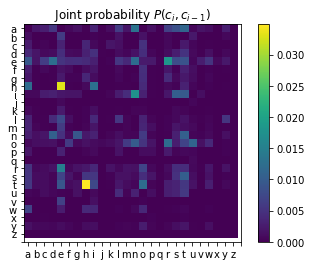
\includegraphics[scale=0.6]{src/5.7 joint probability.png}
    \caption{Joint probability of characters in Metamorphosis.}
\end{figure}
\noindent From the graph above, we can see that \texttt{h} is almost always followed by \texttt{e}. We can make marginal probabilities by summing over the axes.
\begin{figure}[H]
    \centering
    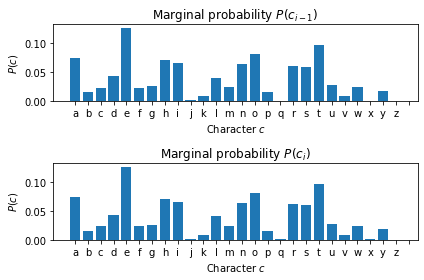
\includegraphics[scale=0.6]{src/5.8 marginal probability.png}
    \caption{Marginal probability of characters in Metamorphosis.}
\end{figure}
\noindent They are almost the same, as they describe pretty much the same PMF (they are only missing 1 sample from the original PMF). We can use also bigraphs to compare the likelihood of one character given the previous character in Metamorphosis.
\begin{figure}[H]
    \centering
    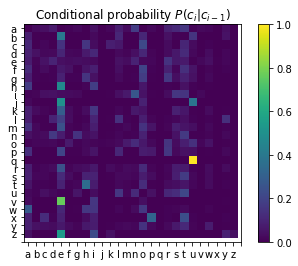
\includegraphics[scale=0.6]{src/5.9 conditional probability.png}
    \caption{Joint probability of characters in Metamorphosis.}
\end{figure}
\noindent Using the bigraph above, we can predict the next character. We can look along the rows to do this look up: each row sums to 1.0. In the \texttt{q} row above, the probability is concentrated on the entry in column \texttt{u}- \texttt{u} always follows \texttt{q} in English.
\newpage

\section{Writing and Manipulating Probabilities}
Probabilities can be used to represent belief. But the raw numbers (e.g. $P(X = x) = 0.9999$) are not always a useful way to make judgments, communicate results, or in some cases, even do computations.

\subsection{Odds and log odds}
The odds of an even with probability $p$ is defined by
\[\operatorname{odds} = \frac{1 - p}{p}.\]
This is easier to understand for unlikely events, e.g. instead of saying the probability is $0.001$, we can say that the odds is $999:1$. Log odds, or logits, are useful for useful for very unlikely scenarios- for a probability $p$, the logit is defined by
\[\operatorname{logit}(p) = \log \left(\frac{p}{1-p}\right).\]
The logit scales proportionally to the number of zeroes in the numerator of the odds. We can display both odds and log odds. Logits (and log probabilities) are more useful when there are multiple magnitudes of data.

If $X$, $Y$ and $Z$ are independent random variables, then $P(X, Y, Z) = P(X) P(Y) P(Z)$. In general, 
\[P(X_1 = x_1, \dots, X_n = x_n) = \prod_{i=1}^n P(X_i = x_i).\]
Since all the probability values are less than 1, multiplying them can lead to underflow errors. So, it is more numrically stable to use log probabilities, i.e.
\[\log P(X_1 = x_1, \dots X_n = x_n) = \sum_{i=1}^n \log P(X_i = x_i).\]
We can also define log likelihood by $\log P(A|B)$. 

% To mean the likelihood of $x_i$, we write $\mathcal{L}(x_i)$. This is not a probability; it is a function of data, and $\mathcal{L}(x_i) = f_X(x_i)$.

Given two observations, we can see whether a third observation is more like the first or the second. We can do this using log likelihoods. For example, if we consider the text Macbeth and compare its character PMF with the log likelihoods of Romeo and Juliet and Metamorphosis PMF, the difference is 113.97- this is positive meaning that it is more like Romeo and Juliet. Instead, if we do the same thing for The Trial, we get $-928.35$. This means that the text is more like Kafka.
\newpage

\section{Bayes' Rule}
\subsection{Prior, likelihood and posterior}
We might want to compute the value $P(A|B)$, but we might only be able to compute $P(B|A)$. In general, $P(A|B) \neq P(B|A)$. We see this kind of issue when:
\begin{itemize}
    \item we want to know the probability of some event given some evidence (e.g. how likely is it that I have a disease given that my blood test came back positive?),
    \item but we only know the probability of observing evidence given the event (e.g. if you have the disease, the blood test will come back positive 95\% of the time).
\end{itemize}
Bayes' Rule can help us invert the probability distribution. It is given by
\[P(A|B) = \frac{P(B|A)P(A)}{P(B)}.\]
We use the following terms to describe the values in the equation above:
\begin{itemize}
    \item $P(A|B)$ is the posterior- what we want to know;
    \item $P(B|A)$ is the likelihood- how likely the event $A$ is to produce the event we see;
    \item $P(A)$ is the prior- how likely the event $A$ is, regardless of the evidence;
    \item $P(B)$ is the evidence- how likely the evidence $B$ is, regardless of the event.
\end{itemize}

If we have some hypothesis $H$, and data $D$, we can rewrite Bayes' rule as:
\[P(H|D) = \frac{P(D|H)P(H)}{P(D)}.\]
To evaluate the equation, we need $P(D)$- the evidence. We can marginalise $P(D)$ from the joint distribution $P(H, D)$ by integrating/summing over all the possible $H$. In particular,
\[P(D) = \sum_i P(D|H_i) P(H_i)\]
for a discrete set of outcomes, and
\[P(D) = \int_A P(D|H) P(H) \ dA\]
for a continuous distribution of outcomes.

Assume that there is a plauge (plauge $X$) spreading all around the world. A new test is developed can detect Plague $X$ with $95\%$ accuracy. We'll assume that $95\%$ accuracy means:
\begin{itemize}
    \item a $5\%$ false positive rule, i.e. $5\%$ of the time people who don't have the disease test positive.
    \item a $5\%$ false negative rule, i.e. $5\%$ of the time people who have the disease test negative.
\end{itemize}
One in one hundred thousand ($1:100 000$) people are known to have Plague $X$. If someone takes the test and the result is positive, then we can compute the likelihood of having the plauge using Bayes' rule.
\small{\begin{align*}
    P(\operatorname{Plague}|\operatorname{Test}) &= \frac{P(\operatorname{Test}|\operatorname{Plague}) P(\operatorname{Plague})}{ P(\operatorname{Test})} \\
    &= \frac{P(\operatorname{Test}|\operatorname{Plague}) P(\operatorname{Plague})}{P(\operatorname{Test}|\operatorname{\lnot Plague})P(\operatorname{\lnot Plague}) + P(\operatorname{Test}|\operatorname{Plague})P(\operatorname{Plague})}.
\end{align*}}
So, after testing positive, one has a $1:5263$ chance of having the plague. Although the test is $95\%$ accurate, the probability of having the plague is very low. This is because so few people have actually gotten the plauge.

Natural frequency explanations involve imagining concrete poulations of a fixed size ($10 000$ people in a room, for example), and considering the proportions as counts (how many people in the room have the plauge?). Bayes' rule is the way to combine evidence- it is used to update the prior belief using observations to get the posterior belief.
\newpage

\section{Entropy}
Entropy is the measure of the ``surprise'' of the result. A flat, uniform distribution is very ``surprising'' because the values are very hard to predict; a narrow, peaked distribution is unsurprising because the values are always very similar.

This is a precise quantification- it gets the information in a distribution. The units of information are normally bits, where 1 bit of information tells us the answer to exactly one yes or no question. The entropy tells us exactly how many of bits are needed (at minimum) to communicate a value from a distribution to an observer who knows the distribution already. Alternatively, we can see the number of distinct states the distribution descrbes as $p = 2^{H(X)}$- this value is called the perplexity, and it can be fractional.

Entropy is given by
\[H(X) = \sum_x -P(X = x) \log_2 P(X = x).\]
It is the expected value of the log-probability of a random variable (the `average' log-probability). 

For example, if a toin coss is unbiased, an observer would have no way of predicting whether the next observation will be heads or tails. Instead, if it is biased, then the observer will be less surprised if their prediction matched the observation. The following image summarises this.
\begin{figure}[H]
    \centering
    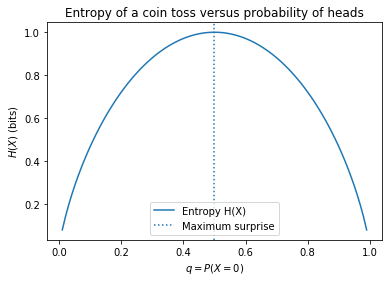
\includegraphics[scale=0.55]{src/5.10 entropy of coin toss.png}
    \caption{Entropy of coin toss as the probability of head changes.}
\end{figure}
\noindent We can also look at the entroy of conditional distribution of characters in Metamorphosis of the next character.
\begin{figure}[H]
    \centering
    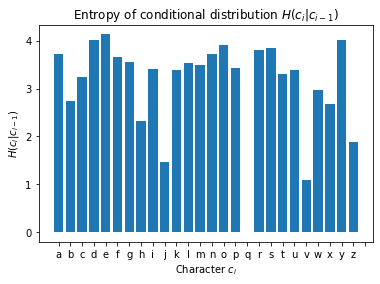
\includegraphics[scale=0.55]{src/5.11 entroy of conditional distribution.png}
    \caption{Entropy of conditional distribution of characters in Metamorphosis.}
\end{figure}
\noindent Most of the time, there is some surprise as to what the next character is. However, if the character is \texttt{q}, then there is no surprise, since the next character is always \texttt{u}.
\newpage

\section{Continuous Random Variables}
\subsection{Problems with continuous random variables}
Continuous random variables are given by probability density functions (PDFs). A PMF is a vector of values, while a PDF is a function that maps any input in the domain to a probability. This results in many complexities:
\begin{itemize}
    \item The probability of a specific value $x$ is always $P(X = x) = 0$, but it is possible that the PDF has support everywhere in its domain (i.e. the value could be this value).
    \item There is no direction way to sample using a PDF.
    \item We cannot estimate the true PDF using empirical observations- this will be finite (i.e. a PMF).
    \item It is not possible to directly apply Bayes' rule on a PMF (every probability is 0).
    \item Simple discrete distributions don't have a concept of dimension. But we can have continuous values in $\mathbb{R}$, or in vector spaces $\mathbb{R}^n$, representing the probability of a random variable taking on a vector value.
\end{itemize}

\subsection{Probability distribution functions}
The PDF $f_X(x)$ of a random variable $X$ maps a value $x$ to a single number- the density at that point. It is a function $\mathbb{R}^n \to \mathbb{R}^+$ ($\mathbb{R}^+$ is the set of positive reals), with
\[\int_x f_X(x) \ dx = 1.\]
While the probability of some outcome with respect to the PDF is at most 1, it is not the case the value $f_X(x)$ is always less than 1.

The probability of the random variable being one value is 0- it is integrating from the value to itself. Instead, we talk about the probability of the random variable being in some range:
\[P(X \in (a, b)) = \int_a^b f_X(x) \ dx.\]
This is illustrated in the figure below.
\begin{figure}[H]
    \centering
    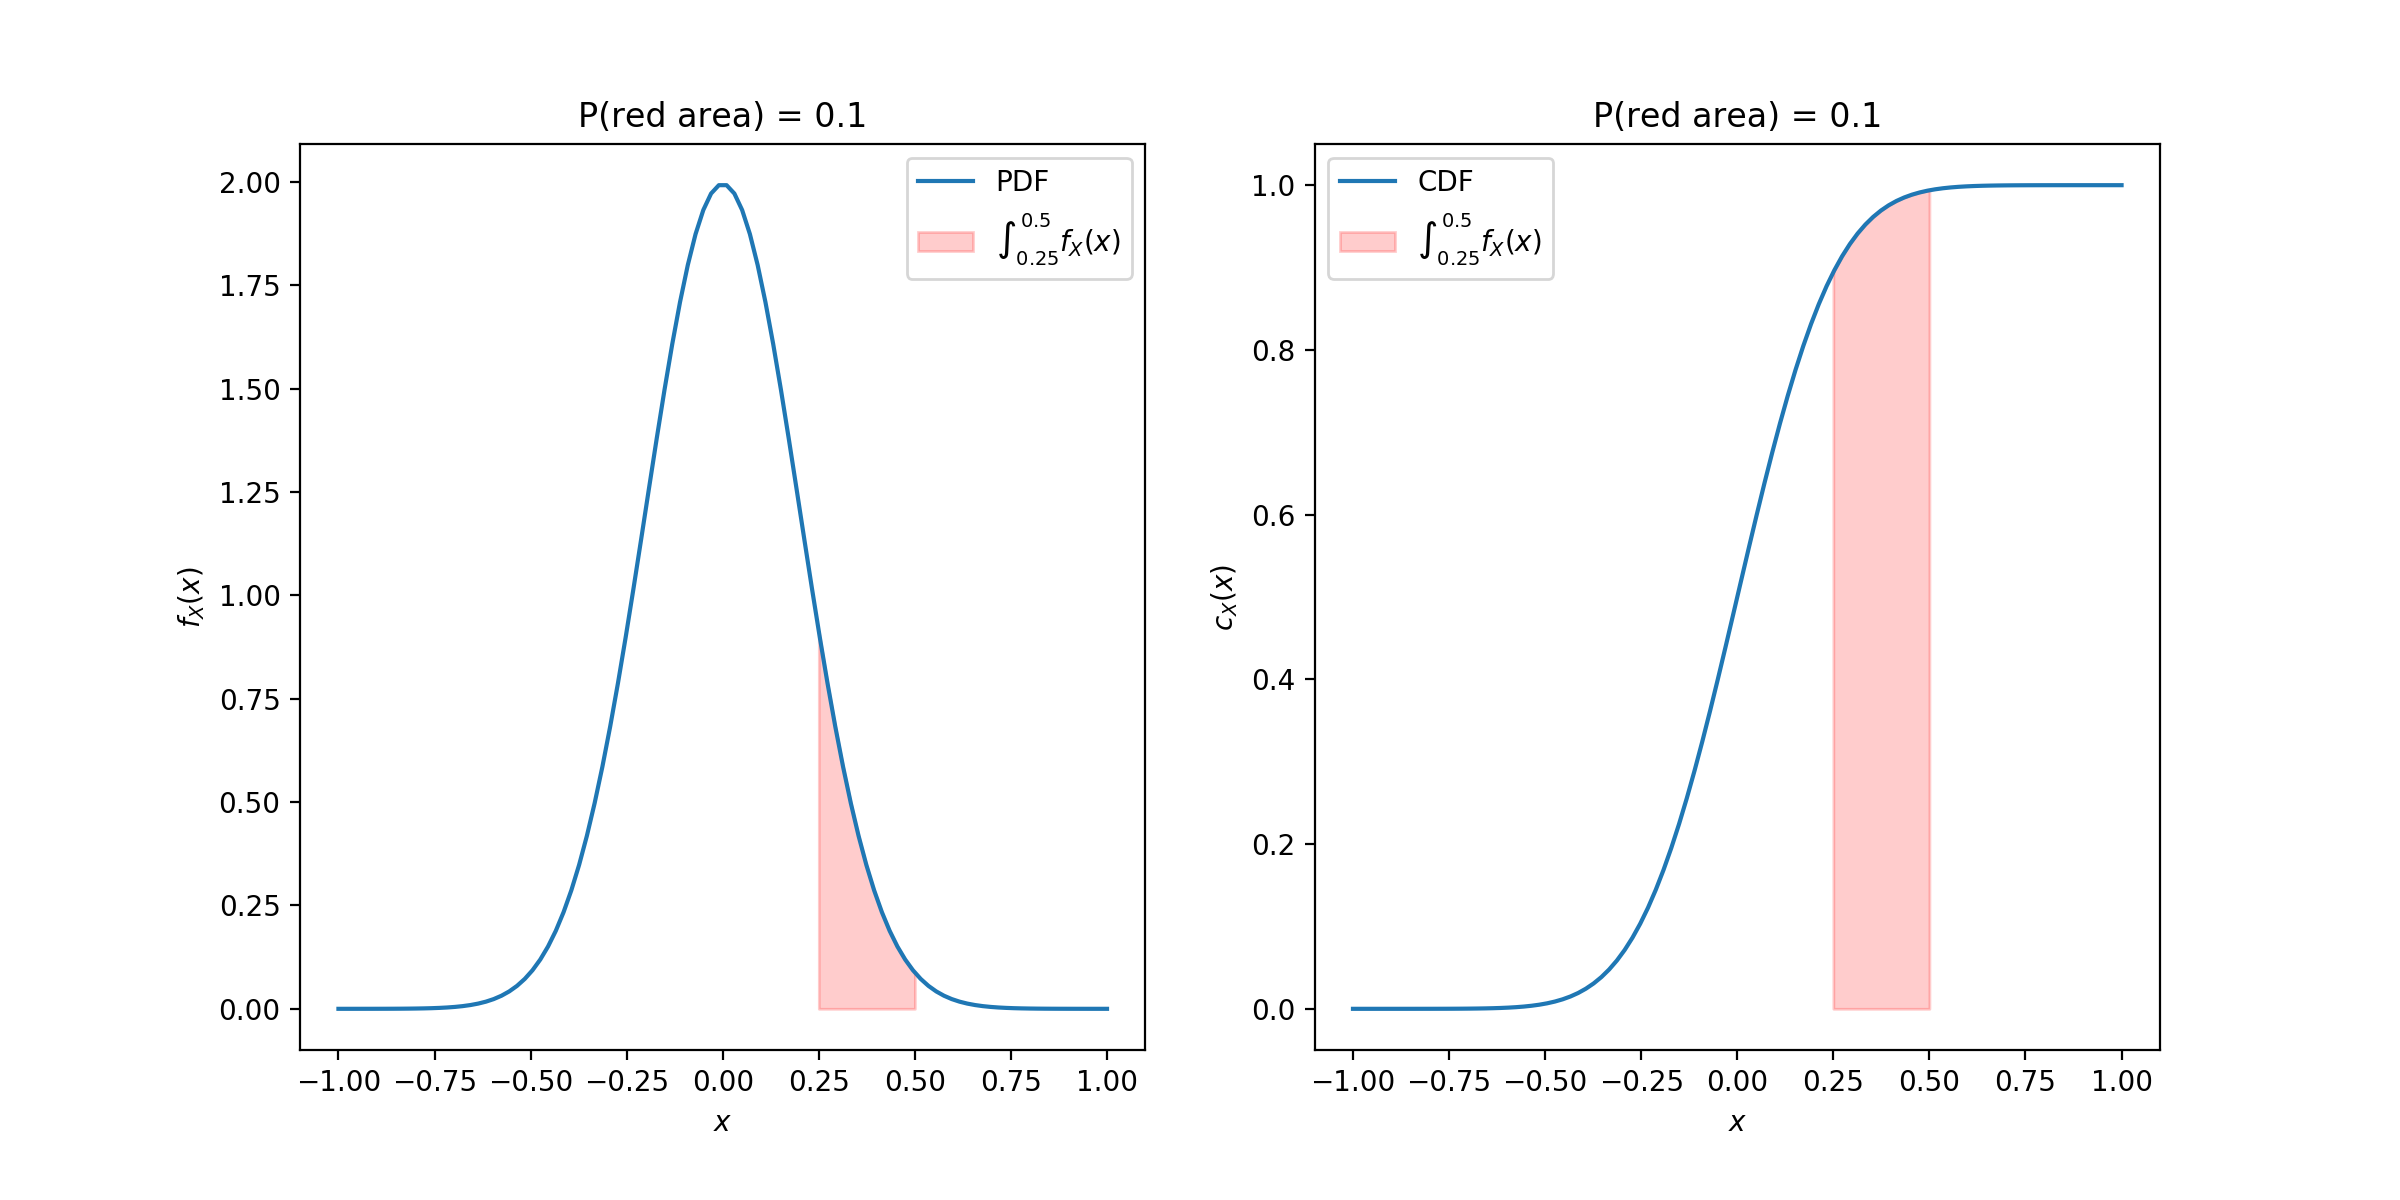
\includegraphics[scale=0.38]{src/5.12 pdf cdf.png}
    \caption{A PDF and its corresponding CDF (cumulative density function).}
\end{figure}
\noindent We have a PDF on the left, and on the right is the corresponding CDF. The red srea gives the probability a value is between 0.25 and 0.5. Note that at 0, the value of the PDF is $2 > 1$.

The support of a PDF is the domain it maps from where the value $f_X(x)$ is not zero, i.e.
\[\operatorname{supp}(x) = \{ x \text{ such that } f_X(x) > 0\}.\]
It is possible to have support just around some interval, and no support everywhere else, e.g. over some interval. This is called compact support. The following PDF has compact support.
\begin{figure}[H]
    \centering
    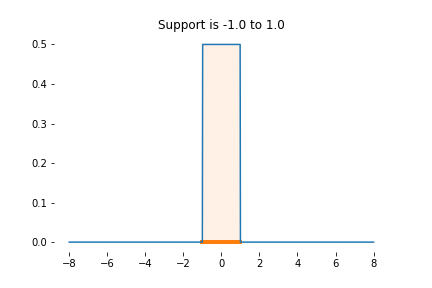
\includegraphics[scale=0.5]{src/5.14 compact support.png}
    \caption{The PDF corresponding to uniform distribution between $-1$ and 1.}
\end{figure}
\noindent There is equal probability for the value to lie between $-1$ and 1- this is uniform distribution. Also, it is possible for a PDF to have support over an infinite domain, e.g. normal distribution. In particular, the following figure illustrates normal distribution around 0.
\begin{figure}[H]
    \centering
    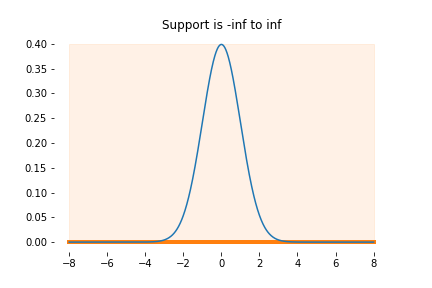
\includegraphics[scale=0.5]{src/5.13 infinite support.png}
    \caption{The PDF corresponding to normal distribution with mean 0.}
\end{figure}
\noindent Sampling using normal distribution could take any value- it is just more likely to pick a value close to the mean of the distribution. This is called infinite support. It is also possible for a function to have semi-infinite support, like in the figure below.
\begin{figure}[H]
    \centering
    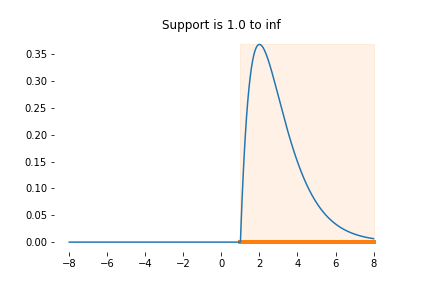
\includegraphics[scale=0.5]{src/5.15 semi infinite support.png}
    \caption{The PDF which has support from 1 to $\infty$.}
\end{figure}

For a PDF, we have a cumulative distribution function (CDF), given by
\[F_X(x) = \int_{-\infty}^x f_X(x) = P(X \leq x).\]
The value of the CDF $F_X(x)$ is always in the range $[0, 1]$. Moreover, it gives us the probability that the random variable will take a value less than or equal to the given value. We can use the CDF to find the probability of the random variable lying in some range, e.g.
\[P(X \in [3, 4]) = F_X(4) - F_X(3).\]
This follows from properties of integration.

\subsection{Normal distribution}
The normal (or Gaussian) distribution is a PDF. It assigns probabilities for every $x \in \mathbb{R}$- it has infinite support. It has density proportional to $e^{-x^2}$ (with some scaling factors so that the integral is $1$). It is called the squared exponential function. We denote $X \sim \mathcal{N}(\mu, \sigma^2)$ to mean that the random variable $X$ is distributed by as normal distribution with mean $\mu$ and variance $\sigma^2$. 

In the normal distribution, the PDF has the highest density at the mean $\mu$- the function decays as we go further from it in both directions. In fact, if the value $x$ isn't within $\sigma$ of the mean, then its density is almost 0. For example, the following figure shows the PDF corresponding to normal distribution with mean 0 and standard deviation 0.5, along with samples taken from it.
\begin{figure}[H]
    \centering
    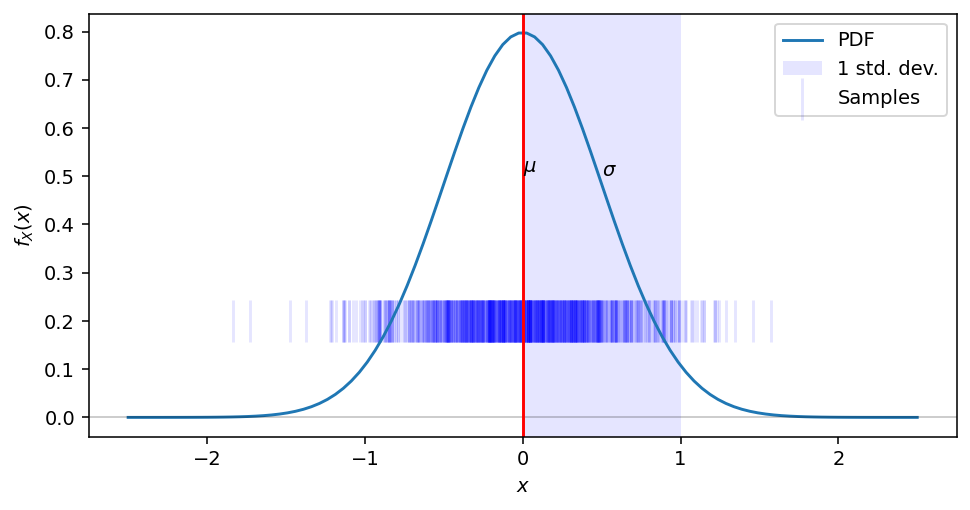
\includegraphics[scale=0.5]{src/5.16 pdf normal distribution.png}
    \caption{The PDF for normal distribution with mean 0 and standard deviation 0.5}
\end{figure}
\noindent Clearly, there is a very high probability around 0, and the value goes down sharply.

Normal modelling has many mathematical properties, and easy to work with analytically (i.e. without relying on numerical computation). Moreover, numerical modelling is applicable most of the time by the central limit theorem.

\subsection{Central Limit Theorem}
If we have a sum of random variables
\[Y = X_1 + X_2 + \dots, \]
then for almost any combination of $X_1, X_2, \dots$, the PDF of $Y$ will be approximately normal. In other words, any process that involves a mixture of many random components will tend to be Gaussian under a wide variety of conditions. For example, consider the emprical PMF for multiple uniform variables.
\begin{figure}[H]
    \centering
    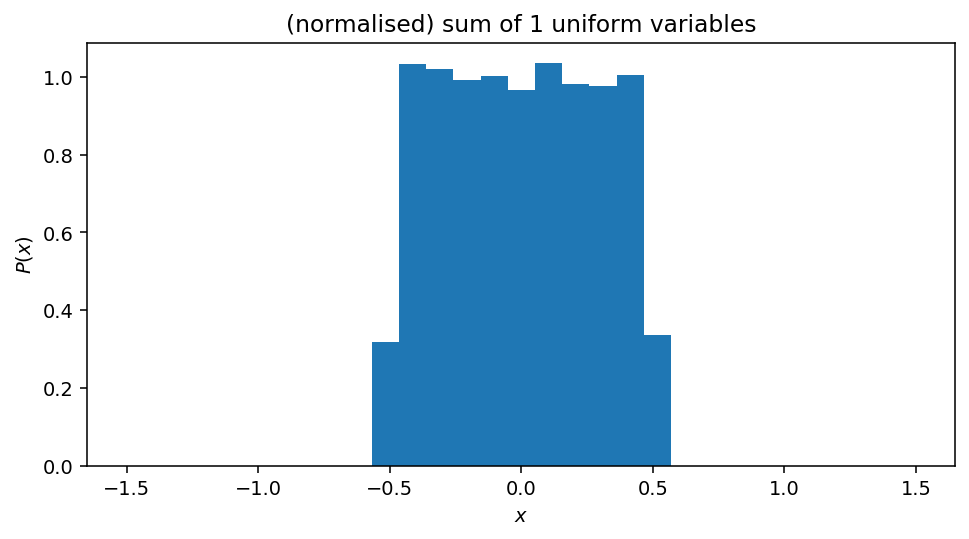
\includegraphics[scale=0.5]{src/5.17 sum of 1 uniform variable.png}
    \caption{The empirical PMF for one uniform variable.}
\end{figure}
\noindent As we expect, the probabilities are uniformly distributed. If we instead have 32 variables, it looks much more like a normal distribution.
\begin{figure}[H]
    \centering
    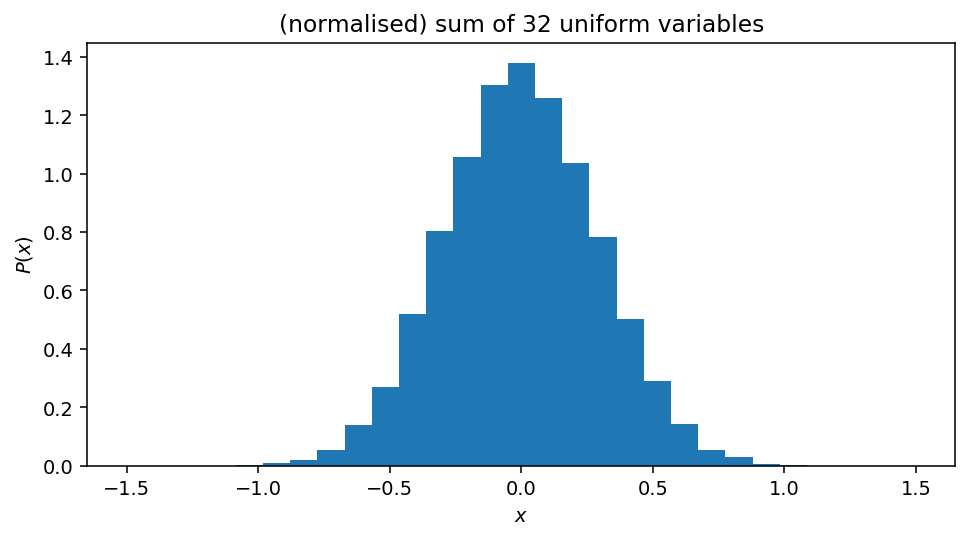
\includegraphics[scale=0.5]{src/5.18 sum of 32 uniform variables.png}
    \caption{The empirical PMF for 32 uniform variables.}
\end{figure}
\noindent In fact, if we had infinitely many uniform variables, the distribution would be perfectly normal.

\section{Multivariate distributions}
Continuous distributions can be generalised from $\mathbb{R}$ to $\mathbb{R}^n$, using PDFs. Like in $\mathbb{R}$, we require
\[\int_{\mathbf{x} \in \mathbb{R}^n} f_X(\mathbf{x}) \ d\mathbf{x} = 1.\]
This is the same as
\[\int_{x_0 = -\infty}^{x_0 = \infty} \int_{x_1 = -\infty}^{x_1 = \infty} \dots \int_{x_n = -\infty}^{x_n = \infty} f_X([x_0, x_1, \dots, x_n]) dx_0 \ dx_1 \ \dots \ dx_n = 1.\]
We can generalise multivariable uniform from uniform distribution in $\mathbb{R}$. For example, the uniform distribution in the box $[0, 1] \times [0, 1]$ in $\mathbb{R}^2$ is:
\begin{figure}[H]
    \centering
    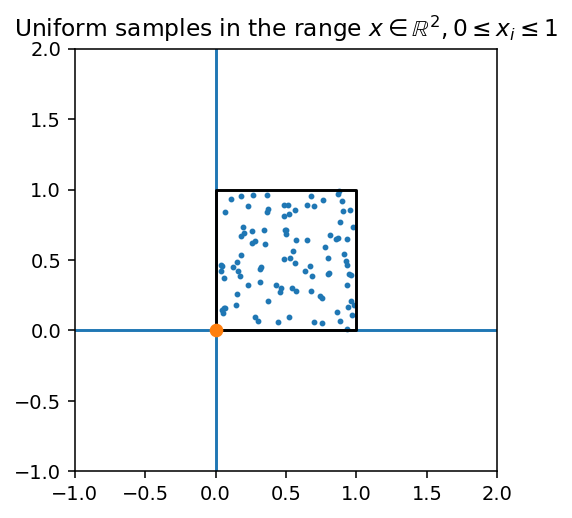
\includegraphics[scale=0.5]{src/5.19 uniform samples in a box.png}
    \caption{Uniform samples in the range $x \in \mathbb{R}^2$, $0 \leq x_1, x_2 \leq 1$.}
\end{figure}
\noindent We can transform this to any area in $\mathbb{R}^2$, using a matrix transformation and a vector offset.
\begin{figure}[H]
    \centering
    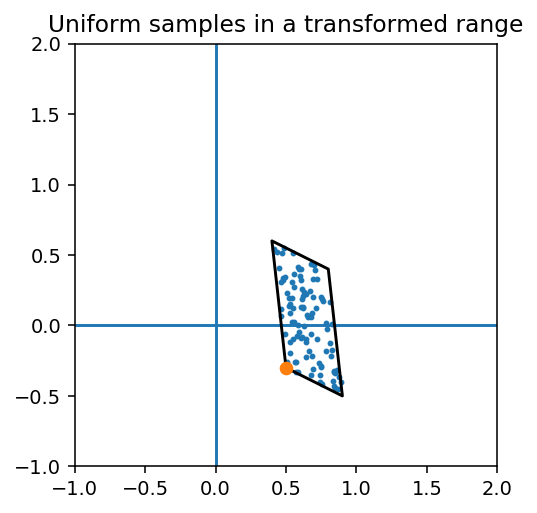
\includegraphics[scale=0.5]{src/5.20 uniform samples in transformed range.png}
    \caption{Uniform samples in a transformed range.}
\end{figure}

We can also generalise normal distribution, using mean $\mu$ and standard deviation $\sigma$ in $\mathbb{R}$ into $\mathbb{R}^n$- using the mean vector $\sigma$ and the covariance matrix $\Sigma$. We can look at the PDF of a multivariate normals for different covariances and mean vector (centres and spreads). For example, normal samples around mean vector $\mathbf{0}$ is the following:
\begin{figure}[H]
    \centering
    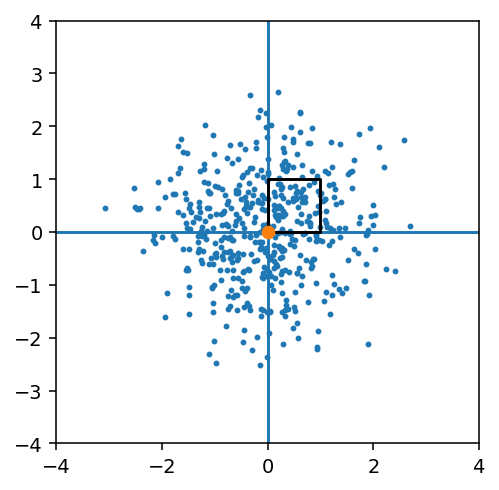
\includegraphics[scale=0.5]{src/5.21 normal spread.png}
    \caption{Normal distribution around the origin in $\mathbb{R}^2$.}
\end{figure}
\noindent The samples are almost circularly spread around the mean. Like in uniform distribution, we can transform this to any area in $\mathbb{R}^2$. Below are some different normal distributions centered at the origin, but with different covariance matrices.
\begin{figure}[H]
    \centering
    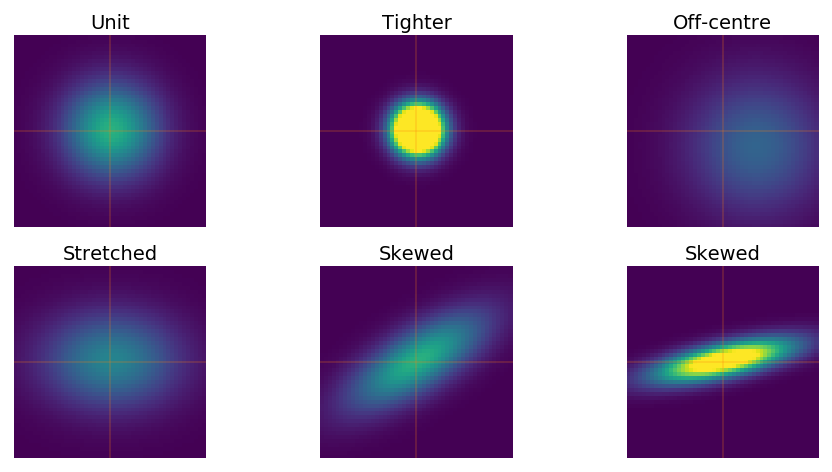
\includegraphics[scale=0.5]{src/5.22 normal distribution examples.png}
    \caption{Different normal distributions in $\mathbb{R}^2$.}
\end{figure}
\noindent We can also talk about the joint probability density function (density over all dimensions) and the marginal probability density function (density over some sub-selection of dimensions). Given a joint probability, we can marginalise it by integrating over one of the axes. An example is shown below.
\begin{figure}[H]
    \centering
    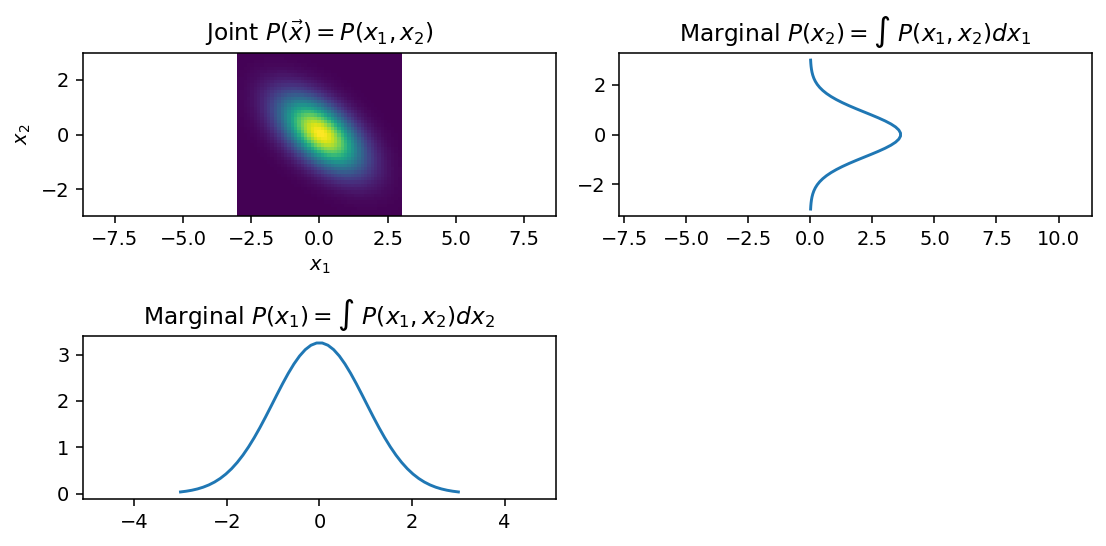
\includegraphics[scale=0.5]{src/5.23 joint and marginal pdf.png}
    \caption{Marginalising the joint PDF by integrating over the two axes.}
\end{figure}
\noindent Now, we can construct the conditional probability for the two random variables.
\begin{figure}[H]
    \centering
    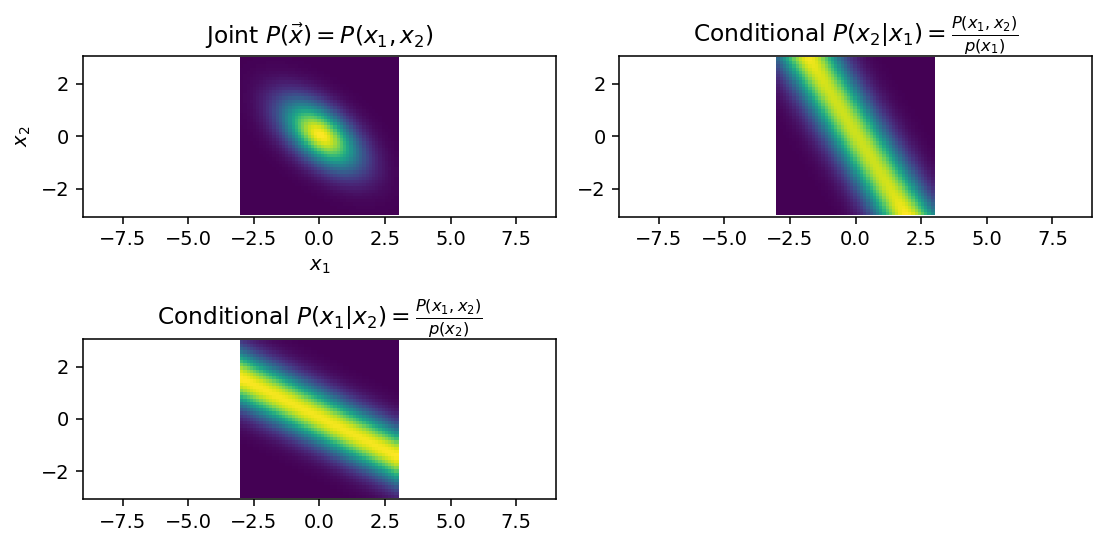
\includegraphics[scale=0.5]{src/5.24 joint and conditional.png}
    \caption{Conditional PDFs for the two random variables above.}
\end{figure}
\noindent When we found an ellipsoidal shape that covered the data, we were finding a covariance matrix and mean vector such that the corresponding normal distribution was shaped like the ellipsoid.

% For example, consider $X \sim \mathcal{N}(\mu, \Sigma)$, where $X \in \mathbb{R}^2$- two dimensional (bivariate) normal distribution. We can consider- joint $P(X)$, marginal ($P(X_1)$ and $P(X_2)$), and conditionals $P(X_1|X_2)$ and $P(X_2|X_1)$)).

% When we spoke informally about the covariance matrix ``covering'' the data with an ellipsoidal shape, we more precisely meant that if we represented the data as being generated with a normal distribution, and choose the mean vector and covariance matrix that best approximated that data, then the contours of the density of the PDF corresponding to equally spaced isocontours would be ellipsoidal.

\section{Monte Carlo}
The Monte Carlo method allows us to (approximately) answer probabilistic problems. It involves setting up a simulation and with stochastic (random) components. By running the simulation many times with different random behaviour, the population of possible behaviours could be approximated.

For example, if we want to compute the expectation of a function of a random variable, we need to compute
\[E[g(X)] = \int_x f_X(x) g(x) \ dx.\]
Since it involves integration, the value might be difficult, if not impossible, to compute. However, it might be easy to compute $g(x)$ for some $x$. So, we can approximated
\[E[g(X)] \approx \frac{1}{N} \sum_{i=1}^N g(x_i),\]
where $x_i$ are random samples from $P(X = x)$, defined by the PDF $f_X(x)$. This gets better as $N$ gets larger.

For example, imagine trying to work out the expectation of dart throw. A dart board has sections giving different scores. We might model the position of the dart as a normal distribution over the dart space. This models the human variability in throwing. The expected score of a throw requires evaluating the integral of the normal PDF multiplied by the score of a throw requires evaluating the integral of the normal PDF multiplied by the score at each point- which isn't feasible to compute directly.

But we can sample from a multivariate normal distribution easily. We can sample $d$ independent standard normals, and transform with a linear transform (i.e. a matrix). So, instead of trying to solve a very hard integral, we can simulate lots of dart throws, which follow the pattern of the normal distribution. We can then take the average score that they get. If we simulate a lot of darts, the average will be close to the true value of the integral. This is the Monte Carlo method. It is very robust and allows us to sample from any PDF. 

% For example, we might want to define a circular score region, which gives us 25 points if we land in it, 50 points if we lie in a small coencentric circle, and 0 otherwise. This is the function $g(X)$. We might model the throw of the dart with a multivariate normal. We compute the expected score $E[g(x)]$ using the Monte Carlo method.

\section{Inference}
Inferential statistics is concerned with estimating the properties of an unobserved ``global'' population of values from a limited set of observed samples. This assumes that there is some underlying distribution from which samples are being drawn. This is a hidden process which we only partially observe through the samples we see.

Population is the unknown set of outcomes (which may be infinite). Sample is some subset of the population that has been observed. So, if we compute the mean from the sample, it will not equal the true mean of the population.

In our model, there is an unknown entity that generates data, according to some definite but unknown rules. These rules are based on some distribution (a type of rule), and parameters (the specifics on the rules applied). We assume the model has some randomness or stochastic elements (as this simplifies the model).

There are three approaches to inference:
\begin{itemize}
    \item Direct estimation of parameters: in this approach, we estimate the values of the parameter directly. For this, we need to know the distribution produced by the generative entity. It is quite efficient, but only works in some cases. In particular, we need estimator function for each specific distribution we want to estimate. An estimator maps observations into parameter estimates.
    \item Maximum likelihood estimation: in this approach, we use optimisation to find the sets of parameters that matches the observations the closest. This uses an iterative optimisation process, but it only works for models where the distribution has a known likelihood function. That is, we need to be able to compute how likely observations were to have been generated by that model.
    \item Bayesian inference: in this approach, we explicitly encode belief about the behaviour of the mysterious entity using probability distributions. In Bayesian models, we assume a distribution over the parameters themselves, and consider the parameters to be random variables. We have some hypotheses (the prior), and we use observations to update these beliefs to make a stronger assumption about the parameters (e.g. a smaller range where the parameter can belong to). We are not estimating a single parameter setting (like in the cases above), but we always have a distribution over the possible parameters. Although this is a more robust and a more coherent way to do inference, it is much harder to represent and compute. We require both priors over parameters, and a likelihood function that will tells us how likely data is to have been generated under a particular parameter setting.
\end{itemize}

We illustrate the approaches by the linear regression problem- given a series of coordinates, find a best-fitting line through them. In particular, we are picking normally distributed points in the line $2x + 9$ in a normally distributed way with standard deviation 3. The following image shows the chosen points.
\begin{figure}[H]
    \centering
    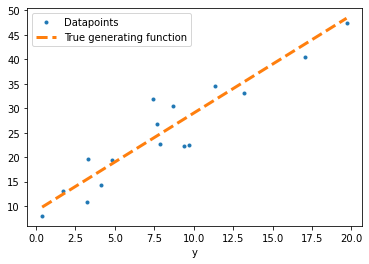
\includegraphics[scale=0.6]{src/5.25 linear regression function.png}
    \caption{Points in the line $2x + 9$ with noise normal distribution (with standard deviation 3).}
\end{figure}
\noindent The true generating function is $2x + 9$. But, the equation of the points is $y = 2x + 9 + \epsilon$, where $\epsilon$ represents the noise. We will assume that $\epsilon \sim \mathcal{N}(0, \sigma^2)$, for standard deviation $\sigma$ (we set it to 3 originally, but we will use this when inferring the equation of the line). So,
\[y \sim \mathcal{N}(mx + c, \sigma^2).\]
Here, $y$ is the random variable, $x$ is known, and we want to infer the gradient $m$, offset $c$ of the line, along with the standard deviation $\sigma$. We can construct a model that generates normally distributed points given $m$, $c$ and $\sigma$, and using inference we can find possible value(s) of $m$, $c$ and $\sigma$.

We cannot estimate empirical distribution directly from observations for PDFs. For many continuous distributions, statisticians have developed estimators; functions that can be applied to sets of observations to estimate the most likely parameters of a PDF defining a distribution that might have generated them. The form of the distribution must be decided in advance (for example, the assumption that the data has been generated by an approximately normal distribution). This is usually called the model. The specific parameters can then be calculated under the assumption of this model.

\section{Direct Estimation}
One way of doing inference is to use estimators of parameters, e.g. if it is normal, use mean and variance of this population distribution. These estimators are computed via statistics which are summarising functions we can apply to data. These estimators need to specially be derived for each specific kind of problem.

For example, the arithmetic mean and the standard deviation of a set of observed samples are statistics which are estimators of the parameters of $\mu$ and $\sigma$ of normal distribution. If we have observations drawn from a normal distribution, we can estimate $\mu$ and $\sigma$ of that distribution just by computing the mean and the standard deviation respectively.

In other words, we might want to know the `true' average brightness- the population mean of the distribution which is `generating' brightness. We have an assumption that a random process is creating these ratings, whose operational characteristics (parameters) we can learn from samples. But, we can only observe a limited sample of ratings by measuring some specific subset of ratings from users who actually rated the app and computing the statistics of the results- the sample mean.

\subsection{Mean}
The arithmetic mean is a sum of sample values $x_1, x_2, \dots, x_n$ divided by the number of values:
\[\hat{\mu} = \frac{1}{N} \sum_{i=1}^N x_i.\]
This is called the sample mean. 

The population mean $\mu$ is the expected value $E[X]$, where $X$ is a random variable. The arithmetic mean $\hat{\mu}$ is a good estimate for $\mu$ in general. The population mean is not normally computable, and is different to the sample mean. However, as we have more samples, we expect it to get closer to the true mean. This is shown in the image below.
\begin{figure}[H]
    \centering
    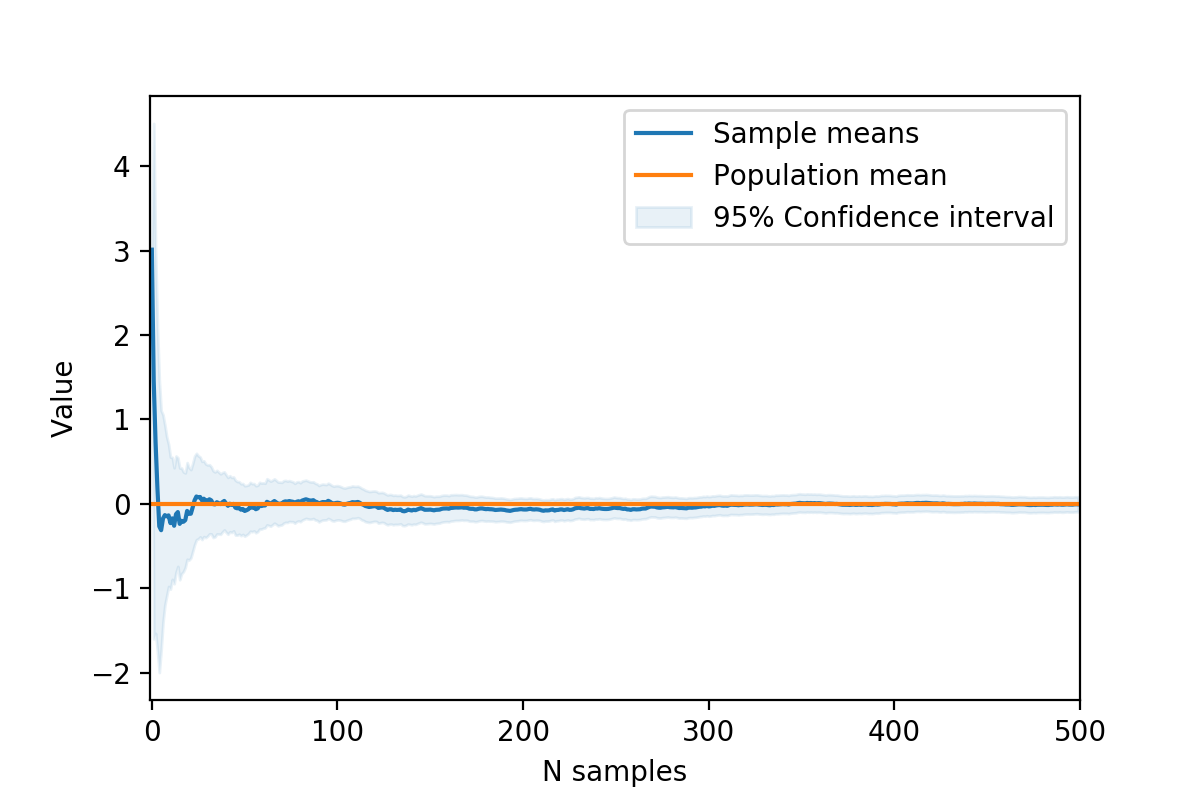
\includegraphics[scale=0.7]{src/5.25 pop_mean.png}
    \caption{How the sample mean changes as the number of samples increases.}
\end{figure}
The sample mean is a statistic (a function of observations), which is an estimator of the population mean (which may be a parameter of the distribution). We can put specific bounds on this estimate; the standard error allows us to measure how close we expect the arithmetic mean of samples is to the population mean, but this interpolation is not straightforward.
The mean scalar measures the central tendency of a collection of values. The mean vector generalises this to higher dimensions.

\subsection{Variance}
The variance of sample values $x_1, x_2, \dots, x_n$ is given by
\[\hat{\sigma}^2 = \frac{1}{N} \sum_{i=1}^N (x_i - \hat{\mu})^2.\]
It estimates the variance $E[(X - E[X])^2]$. This is called the sample variance. The sample standard deviation is the square root
\[\hat{\sigma} = \sqrt{\frac{1}{N} \sum_{i=1}^N (x_i - \hat{\mu})^2}.\]
The variance and the standard deviation measure the spread of a collection values. The covariance matrix $\Sigma$ is the generalisation to higher dimensions. As the number of samples increases, the variance also gets closer to the true sample.

We can use the sample mean and the sample variance to estimate the true mean and the true variance. By the central limit theorem, we know that the data is quite close to normal distribution, so this works quite often. Even if that doesn't apply, the mean and variance are still useful in descriptive statistics.

\subsection{Linear regression}
In direct estimation, we solve linear regression using pseudo-inverses. This gives us an estimate of $m$ and $c$, and we can compute a value for $\sigma$ using the difference of the points and $mx + c$ (i.e. the variance). This gives us the following values:
\begin{itemize}
    \item $m = 2.07$ (actual $m = 2$);
    \item $c = 8.21$ (actual $c = 9$); and
    \item $\sigma = 3.08$ (actual $3$).
\end{itemize}
We can use these values to create the line fit.
\begin{figure}[H]
    \centering
    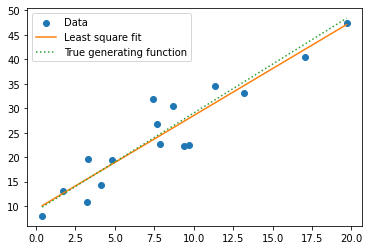
\includegraphics[scale=0.7]{src/5.26 linefit directestimation.png}
    \caption{The line fit for the direct estimator.}
\end{figure}
\noindent We can now sample more points using the inferred values of $m$, $c$ and $\sigma$.
\begin{figure}[H]
    \centering
    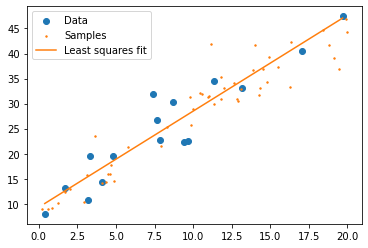
\includegraphics[scale=0.7]{src/5.27 sampling more from direct estimation.png}
    \caption{Sampling more points using the inferred values of $m$, $c$ and $\sigma$ from direct estimator.}
\end{figure}
\noindent This can be used to check whether the inferred values were sensible.

\section{Maximum likelihood estimation}
If we do not have a pre-built estimator that we can use for direct estimation, we can use maximum likelihood estimation. We can typically compute the (log) likelihood of an observation being generated by a specific underlying random distribution. For a PDF, the likelihood of a value $x$ is just the value of the PDF at $x$.

The log-likelihood is the sum of the individual log-likelihoods:
\[\log \mathcal{L}(x_1, x_2, \dots, x_n) = \sum_{i=1}^n f_X(x_i).\]
We can apply optimisation to work out a parameter setting under which the data we actually observed was most likely, using the likelihood function.

If the likelihood depends on some parameters of a distribution $\theta$, then we write $\mathcal{L}(\theta|x)$. Then, we define an objective function- maximising log likelihood, or minimising the negative of log-likelihood. Therefore,
\[\theta^* = \operatornamewithlimits{arg min}_\theta L(\theta),\]
where
\[L(\theta) = -\log \mathcal{L}(\theta | x_1, x_2, \dots, x_n) = -\sum_i \log f_X(x_i, \theta).\]
We assume that $f_X(x_i)$ can be written as $f(x, \theta)$ to represent the PDF of $f$ with some specific choice of parameters given by $\theta$.

The optimisation of negative log-likelihood is called maximum likelihood optimisation. It will find the best setting of parameters that would explain how the observations came to be. We can use any optimisation technique to optimise it, as appropriate. We don't need special estimators in this case, as long as we can evaluate the PDF $f(x, \theta)$ for any setting of parameters $\theta$.

\subsection{Linear regression}
We can do linear regression using maximum likelihood estimation. For this, we need to write the problem in terms of the distribution of random variables. We can think of $y = mx + c$ as a model $Y \sim \mathcal{N}(mx + c, \sigma^2)$- the random variable $Y$ has mean $mx + c$ and standard deviation $\sigma$. To avoid underflow, we will use log likelihood.

In the case where we have normally distributed noise for linear regression, this is exactly equivalent to the direct optmisation with linear least-squares. This is maximum likelihood linear regression. In terms of the objective function, our parameter is $\theta = [m, c, \sigma]$ and objective function computes the log-likelihood that the model $\mathcal{N}(mx + c, \sigma^2)$ produced the given set of results (i.e. the points that we originally had). In particular, for the example of $2x+9+\epsilon$ we had above, with $\epsilon = \mathcal{N}(0, 3)$, MLE gives us the following predictions:
\begin{itemize}
    \item $m = 2.14$ (actual $m = 2$);
    \item $c = 7.19$ (actual $c = 9$); and
    \item $\sigma = 3.14$ (actual $3$).
\end{itemize}
This gives us the following line fit.
\begin{figure}[H]
    \centering
    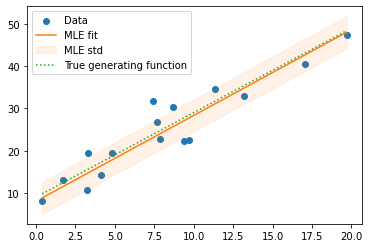
\includegraphics[scale=0.7]{src/5.28 linefit mle.png}
    \caption{The line fit for MLE.}
\end{figure}

\section{Bayesian inference}
In Bayesian inference, we represent the parameters of the distribution as random variables themselves, with distributions of their own. Prior distributions are defined over these parameters (e.g. we might believe that the mean app rating could be any value between 1 and 5, with equal probability), and we use evidence to refine our belief about the distribution of the parameters, using Bayes' rule. We again consider our distribution to be characterise by some parameter vector $\theta$, and we want to refine a distribution over possible $\theta$'s.

Instead of finding the most likely parameter setting, we infer a distribution over possible parameter settings compatible with the data. Given a likelihood $P(D|\theta)$ and prior $P(\theta)$, we can apply Bayes' rule
\[P(\theta|D) = \frac{P(D|\theta) P(\theta)}{P(D)}.\]
This gives us a new distribution over $\theta$ and given some observations. Pictorially, we expect the the prior and the likelihood to affect the posterior as follows:
\begin{figure}[H]
    \centering
    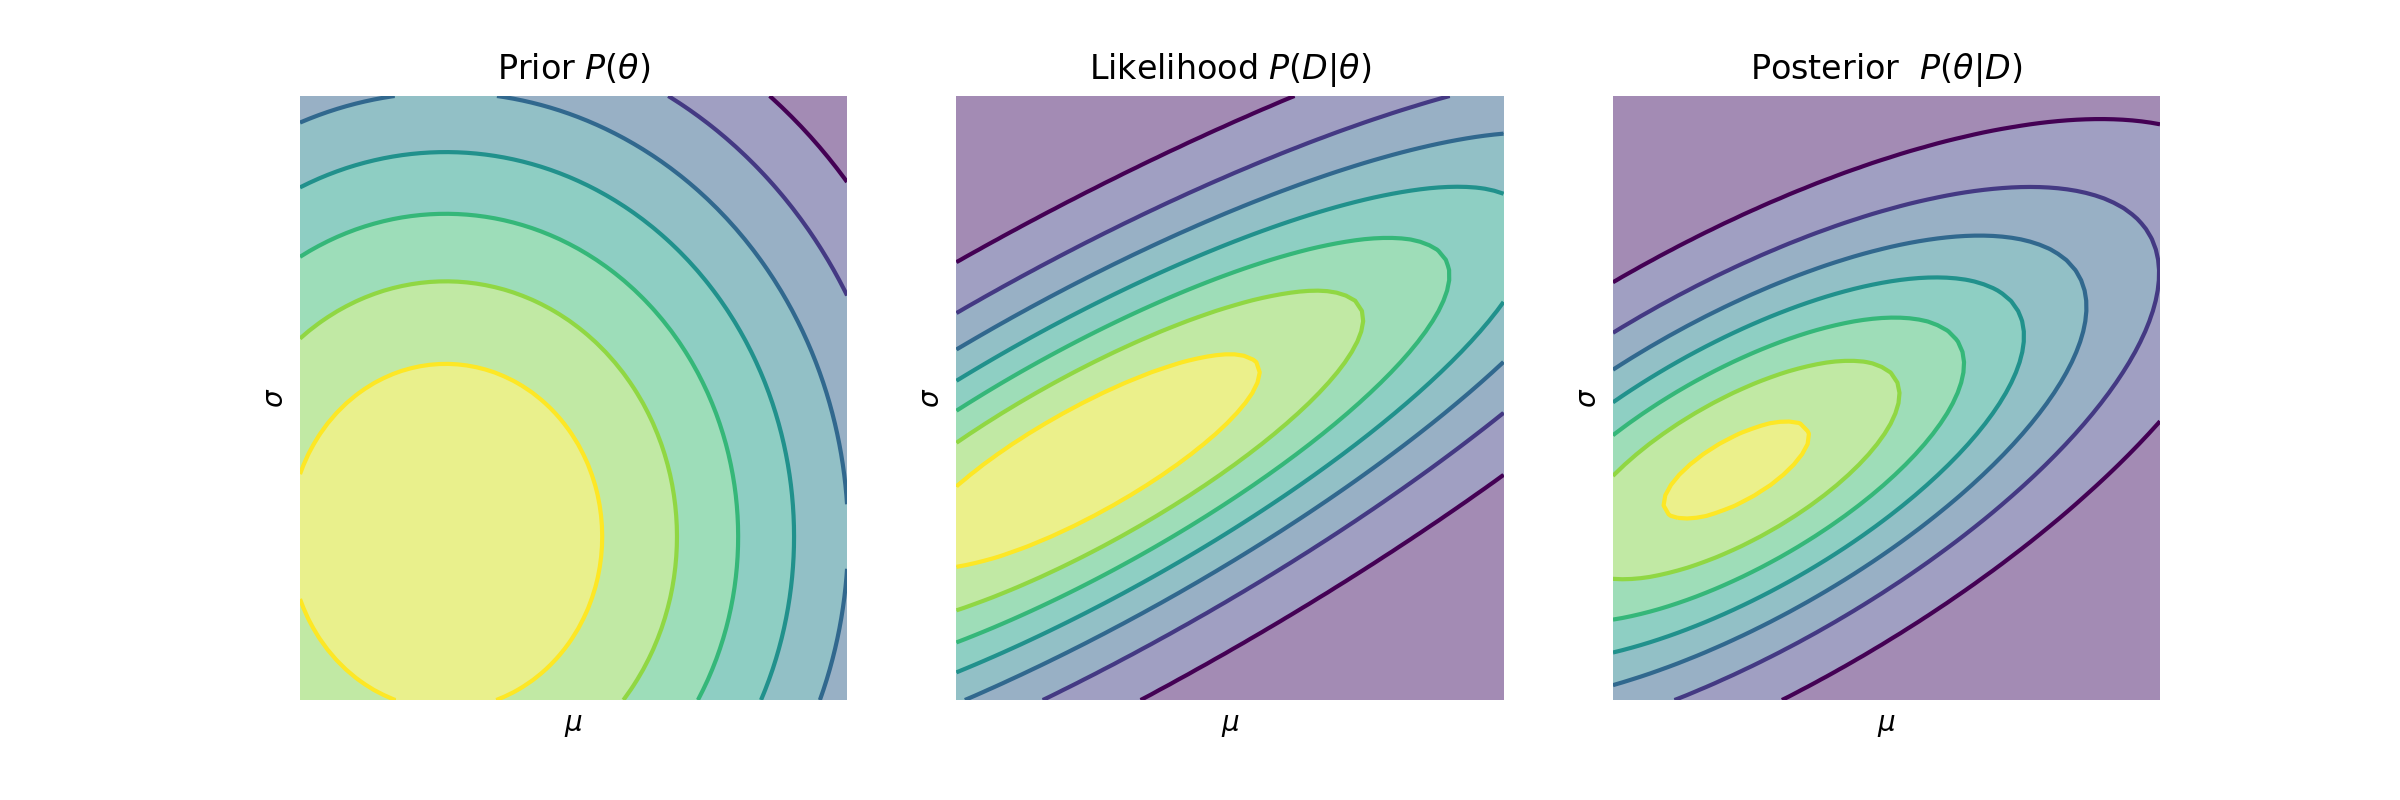
\includegraphics[scale=0.38]{src/5.29 bayesian_inference.png}
    \caption{The process of Bayesian inference- how the prior and the likelihood is used to determine the posterior.}
\end{figure}

Bayes' rule applies to continuous distributions like it did to discrete distributions. However, algebraic computations (i.e. finding results in closed form) are much harder. It is possible in certain cases, but the algebra is often complex and the model choices are limited. When it is possible, it is much more computationally efficient. We will approximate this by drawing samples from the posterior distribution $P(\theta|D)$.

\subsection{Bayesian linear regression}
MLE will give us a possible $m$, $c$ (and $\sigma$), but not how confident we are with it. The Bayesian approach is to let the parameters themselves be random variables. We don't want to optimise. We don't want to find the most likely parameters. We instead want to derive a belief about the parameters as a probability distribution. This is what Bayesians do; they represent belief with probability.

So, if $\theta = [m, c, \sigma]$, we can use Bayes' rule to infer the distribution over it. Here,
\[P(\theta|D) = \frac{P(D|\theta) P(\theta)}{P(D)},\]
where $D$ is the data (an array of coordinates). So, we need:
\begin{itemize}
    \item a prior over the parameters $P(\theta)$. In the linear regression case, we need some initial belief about the possible values of $m$, $c$ and $\sigma$.
    \item a way to calculate the likelihood $P(D|\theta)$.
    \item a way of combining these using Bayes' rule. This is generally impossible, but we can sample from it using Markov Chain Monte Carlo. This will give us samples from the posterior distribution of $P(\theta|D)$ so we can see how sure we should be about our beliefs about the parameters of the mysterious entity.
\end{itemize}
By sampling the parameters $P(\theta)$, we will get different samples for $P(\theta|D)$. This gives us a range of possible line fits that go through the coordinates.

\subsection{Probabilistic programming}
We will use a computational reprsentation where random variables are first-class values and we can write down our models without writing down the detailed mechanics of inference itself. This is probabilistic programming.

We can transform a mathematical expression to a graph. If we have multiple dependent random variables whose distribution we want to infer, we can draw a graph of dependencies between random variables (i.e. ones we don't know the value of precsiely) and inference can be performed on the entire graph. So, we are writing expressions down without fixing the variables, and then allowing the distribution of the values to be inferred when we observe data. This inference narrows down the likely range a random variable could take on.

For example, $y = mx + c$ is modelled as follows:
\begin{figure}[H]
    \centering
    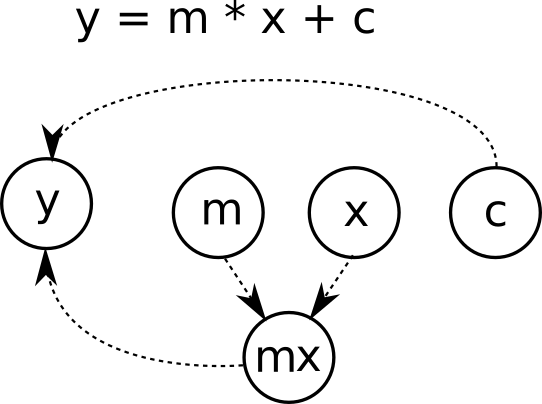
\includegraphics[scale=0.3]{src/5.30 graph model mx+c.png}
    \caption{Graphical model for $y = mx + c$.}
\end{figure}
\noindent Here, some nodes in the graph are observed, while others are unobserved. In particular, the coordinates $(x, y)$ are observed, but the parameters $m$, $c$ and $\sigma$ are not observed. We can infer the posterior distribution of unobserved nodes by integrating over the possible values that could have occurred given the observed values.

We need to specify that $y$ is normally distributed with mean $mx + c$ and spread $\sigma$, and we can infer these values from the coordinates. So, the model with dependencies and observence is given below.
\begin{figure}[H]
    \centering
    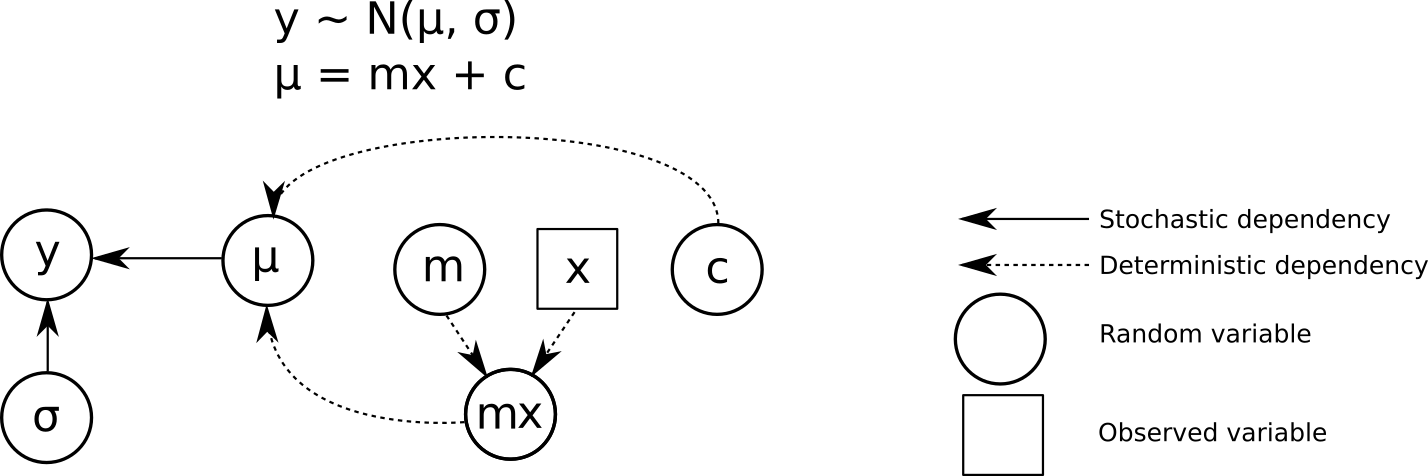
\includegraphics[scale=0.3]{src/5.31 linear regression model.png}
    \caption{Graphical model for $y = mx + c$ with dependency and observence.}
\end{figure}
\noindent A deterministic dependency means that finding the dependencies fully determines the value, e.g. knowing $m$ and $x$ fully determines the value $mx$. On the other hand, a stochastic dependency means that finding the dependencies still leaves some randomness to the value, e.g. knowing $\mu$ and $\sigma$ doesn't mean we know what $y$ is- we just know what range it is likely to lie in.

Our assumption here is that we will observe data which has a latent structure modelled by a linear dependence on a variable $x$, plus some normally-distributed observation noise. To apply Bayes' rule, we need to have some prior distribution on every stochastic node (i.e. $m$, $c$ and $\sigma$, but not $mx$). We can't have any ``wild'' stochastic nodes which do not eventually depend on deterministic nodes, via some chain of prior distributions.

We want to infer a distribution over $m, c, \sigma$, and not a distribution over the observations. That is, we will treat the parameters themselves as random variables, with their own distributions, and use Bayesian reasoning (i.e. applying Bayes' rule) to infer a posterior distribution over the parameters given some prior, and some evidence observed. We expect the posterior distribution to be much tighter than the prior distribution.

Given a prior and a likelihood and some observations, we can draw samples from the posterior $P(\theta|D)$. the issues here are:
\begin{itemize}
    \item we need $P(D|\theta)$ for a distribution over $\theta$, not just a few numbers. We need a closed form for the distribution function.
    \item the value $P(D) = \int_\theta P(D|\theta) P(\theta) \ d\theta$, which is quite difficult (if not impossible) to compute.
\end{itemize}
However, for a fixed $\theta = [m, c, \sigma]$, it is often trivial to compute $P(\theta|D)$. This is because we can easily compute $P(D)$ and $P(D|\theta)$ in that case. This can be thought of as drawing samples from the posterior distribution $P(\theta|D)$, instead of computing the distribution exactly.

We can also simplify this by only focusing on the relative probability of different parameter settings with the data $D$. In that case,
\[P(\theta|D) \propto P(D|\theta) P(\theta).\]
This only makes sense because we are only considering one model with one set of data in this example.

\section{Markov Chain Monte Carlo}
We can implement a procedure to sample from the relative posterior distribution. This defines a random walk through the space of parameter settings, proposing small random tweaks to the parameter settings, and accepting ``jumps'' if they make the estimate more likely, or with a probability proportional to the change in $P(D|\theta) P(\theta)$ if not. This means we can use samples from $\theta$ and not integrate. This is called Markov Chain Monte Carlo (MCMC). To evaluate this, we need $P(D|\theta)$ (likelihood) and $P(\theta)$ (prior) for a given $\theta$.

MCMC allows us to run inference after writing down the model. However, the sampling strategy has a very large influence for the kind of sample runs that are practical to execute. True Bayesian inference depends only on the prior and the evidence. MCMC also depends on the sampling strategy used to approximate the posterior.

The equation we use is
\[P(\theta|D) \propto P(D|\theta) P(\theta),\]
where $P(\theta|D)$ is the posterior, $P(D|\theta)$ is the likelihood and $P(\theta)$ is the prior. We ignore the eveidence $P(D)$ as a normalising constant. In Python, we can use \texttt{PyMC3} to do inference.

In the linear regression model, the set of observations $D$ is an array of coordinates. We represent the distribution parameters as $\theta = [m, c, \sigma]$, and can talk about $P(\theta|D)$, a probability distribution over the parameter vectors. Our prior beliefs are:
\begin{itemize}
    \item $m \sim \mathcal{N}(0, 50)$;
    \item $c \sim \mathcal{N}(0, 50)$; and
    \item $\sigma \sim U(0.01, 100)$.
\end{itemize}
These are very weak assumptions. Next, we define the likelihood function. This is a function of the data given some parameter setting, and is the same as the MLE in this case. The likelihood of one sample is just the normal PDF evaluated at that point, and the likelihood of all samples is the product of these likelihoods.
\[L(D|\theta) = L(x, y; m, c, \theta) = f_X(y - mx + c, \sigma^2).\]
We can then sample from the model. We need to specify how many samples to take from the posterior predictive $P(\theta|D)$. This gives us a range of distributions for $m$, $c$ and $\sigma$, with 500 samples:
\begin{figure}[H]
    \centering
    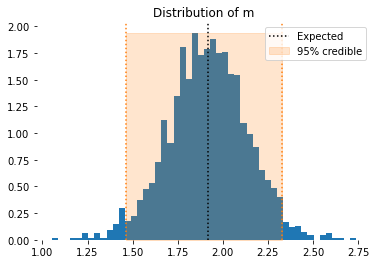
\includegraphics[scale=0.5]{src/5.32 distribution of m.png}
    \caption{Distribution of $m$.}
\end{figure}
\begin{figure}[H]
    \centering
    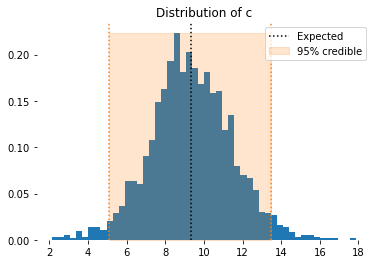
\includegraphics[scale=0.5]{src/5.33 distribution of c.png}
    \caption{Distribution of $c$.}
\end{figure}
\begin{figure}[H]
    \centering
    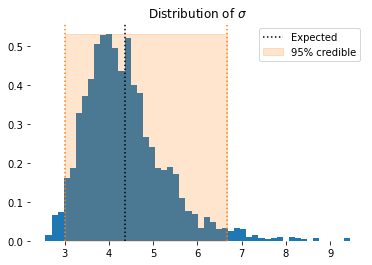
\includegraphics[scale=0.5]{src/5.34 distribution of sigma.png}
    \caption{Distribution of $\sigma$.}
\end{figure}
\noindent We have quantified uncertainty- because our sample size was quite low (just 16), we cannot say with confidence that the value of $m$ is 1.9. This is an advantage of Bayesian inference. Also, with more samples, our confidence on the distributions will increase. We can plot the 500 predictions of the regression lines as well. 
\begin{figure}[H]
    \centering
    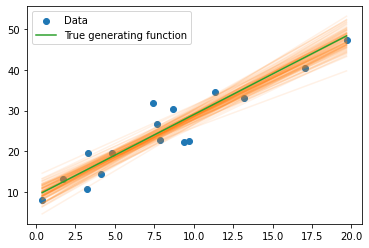
\includegraphics[scale=0.6]{src/5.35 linefits bayesian.png}
    \caption{Possible line fits for Bayesian linear regression.}
\end{figure}

In summary, we are doing the following:
\begin{itemize}
    \item we infer parameters of the model in the form of samples (definite values for the parameters);
    \item we can then use those definite values to simulate behaviour using our linear model;
    \item this given us a collection of simulations;
    \item we can plot all of these overlaid.
\end{itemize}

\subsection{Predictive Posterior}
We predicted the line fits with the posterior distributions of $m$, $c$ and $\sigma$. These are the values we expect the model parameters to take on, given the data we observed (likelihood) and our prior. We had also set prior distributions of $m$, $c$ and $\sigma$. We could plot these as well.
\begin{figure}[H]
    \centering
    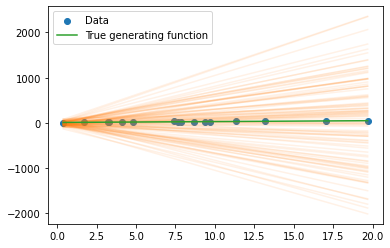
\includegraphics[scale=0.6]{src/5.36 linefit bayesian prior.png}
    \caption{Prior line fits for Bayesian linear regression.}
\end{figure}
\noindent Thes are much less accurate because our initial guess allowed for a lot more configurations of $m$, $c$ and $\sigma$.

The predictive posterior is the distribution over observations we would expect to see. We draw samples from the model, while integrating over parameters from the posterior. By sampling from the predictive posterior, we are generating new synthetic data that should have the same statistical properties as the data (if our model is good).

In the linear regression example, the predictive posterior tells us the likely values of $y$ using the posterior distribution of $m$, $c$ and $\theta$. The following histogram shows the predictive posterior and the prior posterior.
\begin{figure}[H]
    \centering
    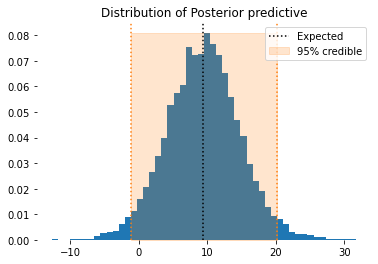
\includegraphics[scale=0.6]{src/5.37 posterior predictive.png}
    \caption{Posterior predictive.}
\end{figure}
\begin{figure}[H]
    \centering
    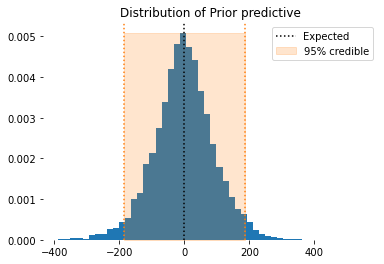
\includegraphics[scale=0.6]{src/5.38 prior predictive.png}
    \caption{Prior predictive.}
\end{figure}

\end{document}